\documentclass[10pt]{report}

\usepackage{talks}
\newcommand{\expect}[1]{\mathbb{E}\!\left[ #1 \right]}
\newcommand{\reals}{\mathbb{R}}
\newcommand{\draw}[2]{#1^{(#2)}}
\usepackage{mathpazo}
\usepackage{sourcecodepro}
\usepackage{tikz}
    \usetikzlibrary{positioning, shapes, arrows.meta}

\begin{document}

\sf \mbox{}
\\[12pt]
\spc{\LARGE\bfseries \color{MidnightBlue}{Multiscale MCMC sampling}}
\\[4pt]
\spc{\Large\bfseries \color{MidnightBlue}{with delayed rejection
    generalized HMC}}
\\[24pt]
\noindent 
\spc{\large\bfseries \color{MidnightBlue}{Bob Carpenter}}
\\[2pt]
\spc{\small Center for Computational Mathematics}
\\[-1pt]
\spc{\small Flatiron Institute}
\\[2pt]
\spc{\footnotesize \url{bcarpenter@flatironinstitute.org}}
\vfill 
\noindent 
\spc{\footnotesize September 2023 \qquad University of Michigan SciML Webinar}
\hfill

\includegraphics[width=1.25in]{img/flatiron-logo.eps}


\sld{The problem and the solution}
\begin{itemize}
\item \myemph{Goal}: Bayesian posterior inference for multiscale
  posteriors
\item \myemph{Measure of curvature}: Spectrum (eigenvalues) of Hessian
  (2nd derivative matrix) of log posterior density 
\item \myemph{Multiscale}: Spectrum varies with parameters
  \begin{subitemize}
    \item \myemph{Examples}: hierarchical prior for varying effects, stochastic
      volatility models, ODEs of varying stiffness w.r.t.\ parameters,
      etc.
    \end{subitemize}
  \item \myemph{Problem}: \myemph{0th order} (Gibbs, RWM) and \myemph{1st
        order} (MALA, HMC, NUTS) methods fail
      \myemph{2nd order} (Riemannian HMC) is too expensive in high dimensions
\item \myemph{Solution}: multiscale integrator (generalized HMC with
  delayed rejection)
\end{itemize}

\sld{Bayesian quantities of interest are expectations}
\begin{itemize}
\item \myemph{Posterior} $p(\theta \mid y) \propto p(y \mid \theta) \cdot
  p(\theta)$ with \myemph{data} $y$ and \myemph{parameters} $\theta \in \mathbb{R}^D$.
\item \myemph{Parameter estimate} minimizing expected square error:
  $$ \textstyle
  \widehat{\theta}
  = \expect{\theta \mid y}
  = \int_{\mathbb{R}^D}
  \theta \cdot p(\theta \mid y)
  \, \textrm{d}\theta 
  $$
\item \myemph{Event probability} for event $A \subseteq \mathbb{R}^D$:
  $$ \textstyle
  \Pr[A \mid y]
  = \expect{\textrm{I}(\theta \in A) \mid y}
  = \int_{\mathbb{R}^D}
  \textrm{I}(\theta \in A) \cdot p(\theta \mid y) 
  \, \textrm{d}\theta 
  $$
\item \myemph{Posterior predictive density} for new data $\widetilde{y}$:
  $$ \textstyle
  p(\widetilde{y} \mid y) 
  = \expect{p(\widetilde{y} \mid \theta) \mid y}
  = \int_{\mathbb{R}^D}
  p(\widetilde{y} \mid \theta) \cdot p(\theta \mid y) 
  \, \textrm{d}\theta 
  $$
\end{itemize}


\sld{Monte Carlo integration in high dimensions}
\begin{itemize}
\item Given a Bayesian \myemph{posterior density} $p(\theta \mid y),$
  with support for \myemph{parameters} $\theta \in \mathbb{R}^D$ and \myemph{data} $y$,
  draw a \myemph{sample}
  $$ \textstyle
  \draw{\theta}{1}, \ldots \draw{\theta}{M} \sim p(\theta \mid y)
  $$
\item to evaluate \myemph{posterior expectations} of functions $f$
\begin{align*}
  \textstyle 
  \expect{f(\theta) \mid y}
  &= \textstyle \int_{\mathbb{R}^D} f(\theta) \cdot p(\theta \mid y) \,
    \textrm{d}\theta
  \\[4pt]
  &= \textstyle \lim_{M \rightarrow \infty} \frac{1}{M} \sum_{m=1}^M 
f\left( \draw{\theta}{m} \right)
  \\[4pt] \textstyle
  &\approx \textstyle \frac{1}{M} \sum_{m=1}^M f\left(\draw{\theta}{m}\right) 
\end{align*}
\end{itemize}

\sld{Hessians are second derivatives}
\begin{itemize}
\item Given a posterior density $p(\theta \mid y),$ its \myemph{Hessian} is the
  matrix of \myemph{second (partial) derivatives},
  $$
  \textrm{H}(\theta) = \nabla_{\!\!\theta} \, \nabla_{\!\!\theta}^\top \ p(\theta \mid y).
  $$
  with entries
  $$
  \textrm{H}_{i, j}(\theta) = \frac{\partial^2}{\partial \theta_i \, \partial
    \theta_j} p(\theta \mid y).
  $$
\item If $p(\theta \mid y) = \textrm{normal}(\theta \mid \mu, \Sigma)$ with
  \myemph{positive definite covariance} $\Sigma$, then the Hessian is the
  negative inverse covariance (i.e., negative precision),
  $$
  \textrm{H}(\theta) = -\Sigma^{-1}.
  $$
\item 
  
  $\Sigma = \textrm{diag}([\sigma_1^2 \cdots \sigma_D^2])$ is
  \myemph{diagonal}, then its Hessian is $\textrm{diag}([\sigma_1^{-2} \cdots
  \sigma_D^{-2}])$
\end{itemize}

\sld{The spectrum of eigenvalues}

\begin{itemize}
\item If $A$ is a $D \times D$ matrix, its \myemph{eigendecomposition} is
  $$
  A = Q \cdot \textrm{diag}(\lambda) \cdot Q^{-1}
  $$
  $\lambda$ a $D$-vector of \myemph{eigenvalues}, $Q$ a
  $D \times D$ orthonormal matrix of \myemph{eigenvectors}
\item Eigenvalues are \myemph{inverse squared scales} in the direction of the eigenvalues
\end{itemize}

\sld{Positive definiteness and log concavity}
\begin{itemize}
\item A matrix is \myemph{positive definite} if the eigenvalues are
  all positive
\item A density is \myemph{log concave} at a point if its Hessian is positive definite. 
\item A multivariate normal with \myemph{diagnonal covariance} $\Sigma =
  \textrm{diag}([\sigma_1^2 \cdots \sigma_D^2])$ has
  \begin{subitemize}
    \item axis-aligned eigenvectors, $Q = \textrm{I}$ ($\textrm{I}$ is
      identity)
    \item eigenvalues $\lambda = \sigma_1^{-2}, \ldots, \sigma_D^{-2}$
  \end{subitemize}
\item Eigenvalues are \myemph{rotation invariant}.
\item For non-diagonal covariance, just \myemph{rotate to diagonal}.
\end{itemize}

\sld{Condition numbers and iterative algorithms}
\begin{itemize}
\item The \myemph{condition} of a positive definite matrix $A$ is the 
  ratio of largest to smallest eigenvalue,
  $$c = \frac{\max(\lambda)}{\min(\lambda)}.$$
\item To move a ``unit,'' gradient-based algorithms take \myemph{steps
    proportional to smallest scale} and a \myemph{number of steps
    equal to the condition}.
\item A posterior $p(\theta \mid y)$ has
  \begin{subitemize}
    \item \myemph{varying curvature} if its Hessian changes for
      different
    $\theta$, and
    \item \myemph{varying scale} if its smallest scale changes for
      different $\theta$.
  \end{subitemize}
\item Thus \myemph{varying scales require varying step sizes} (for
  gradient-based algo).
\end{itemize}

\sld{Neal's funnel as a proxy for hierarchical priors}
\begin{itemize}
  \item Neal's funnel for log scale (times two) $y \in \mathbb{R}$ and
    varying effects $x \in \mathbb{R}^N$ is
    $$ \textstyle 
    p(x, y) = \textrm{normal}(y \mid 0, 3) \cdot \prod_{n=1}^N 
    \textrm{normal}(x_n \mid 0, \exp(y / 2)). 
    $$
    \begin{center}
      \vspace*{-9pt}
    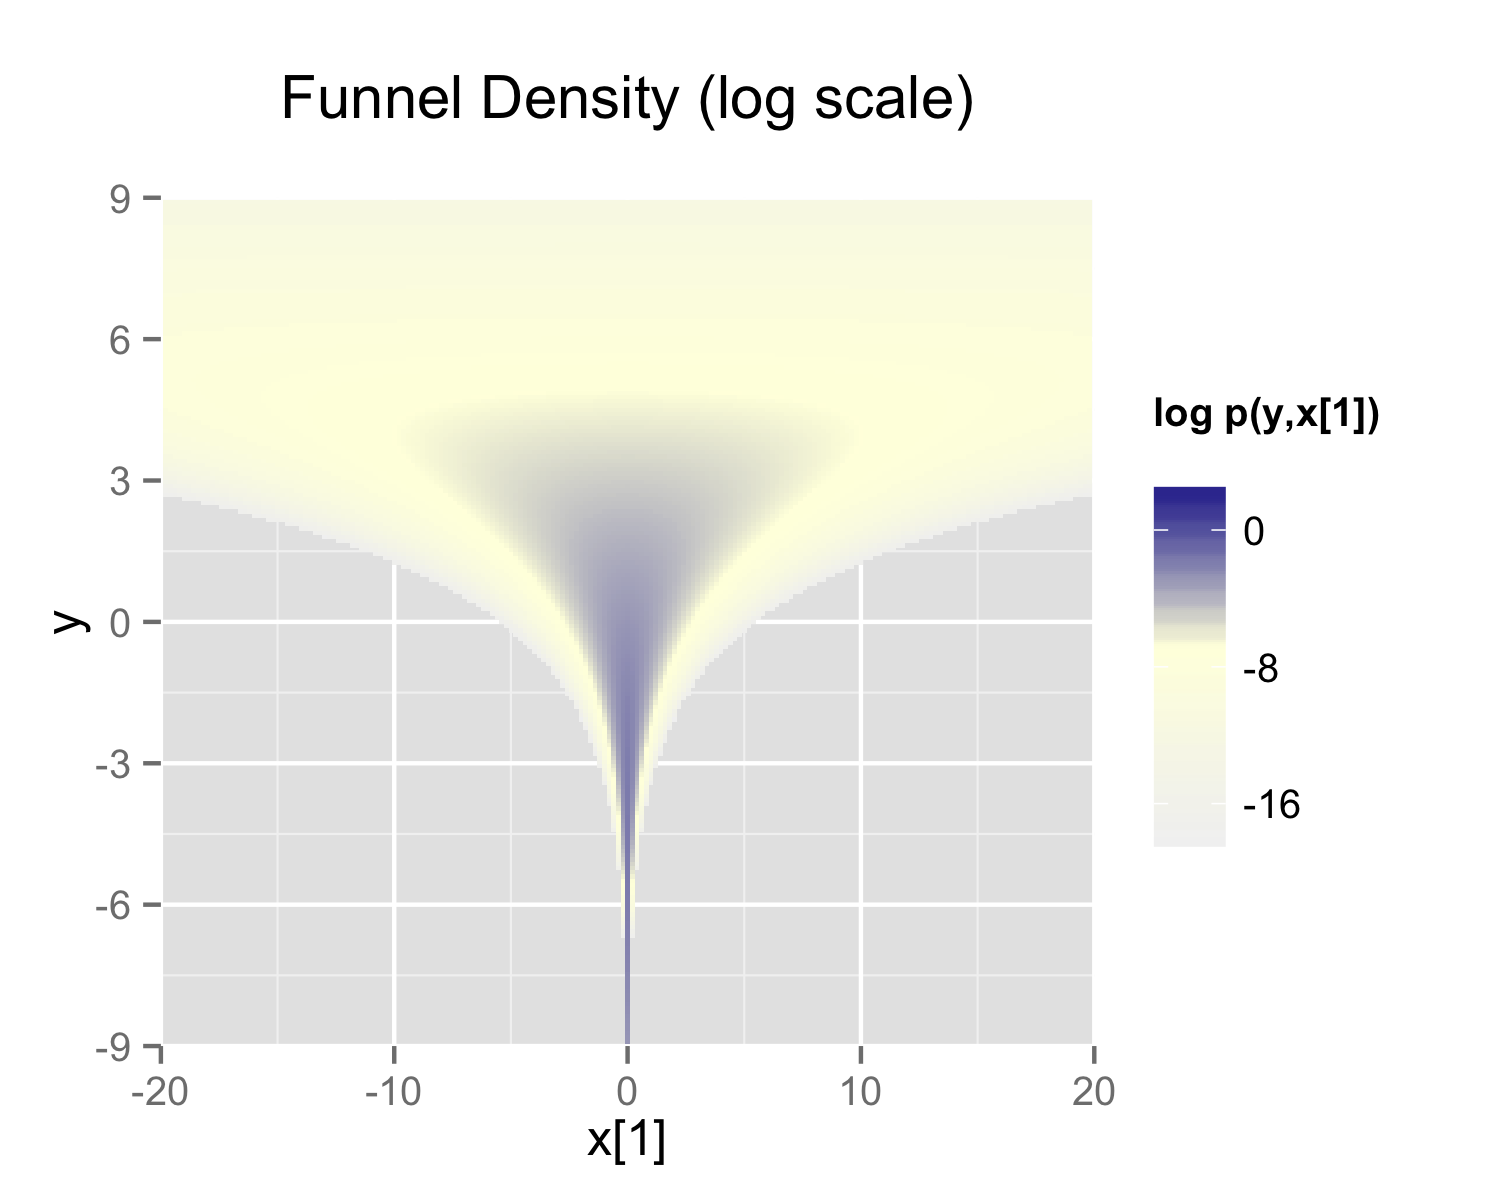
\includegraphics[width=2.25in]{img/funnel.png}
  \end{center}
\end{itemize}

\sld{Neal's funnel has varying curvature and scale}
\begin{itemize}
\item Here's a plot of the (rotated) funnel and its condition number
  vs.\ scale $\beta$
\item central 95\% interval for constant scale $\beta$---condition
  worsens in tails
\item Eigenvectors change orientation (biggest along $\beta$ in neck,
  along $\alpha$ in mouth)
\end{itemize}
\begin{center}
  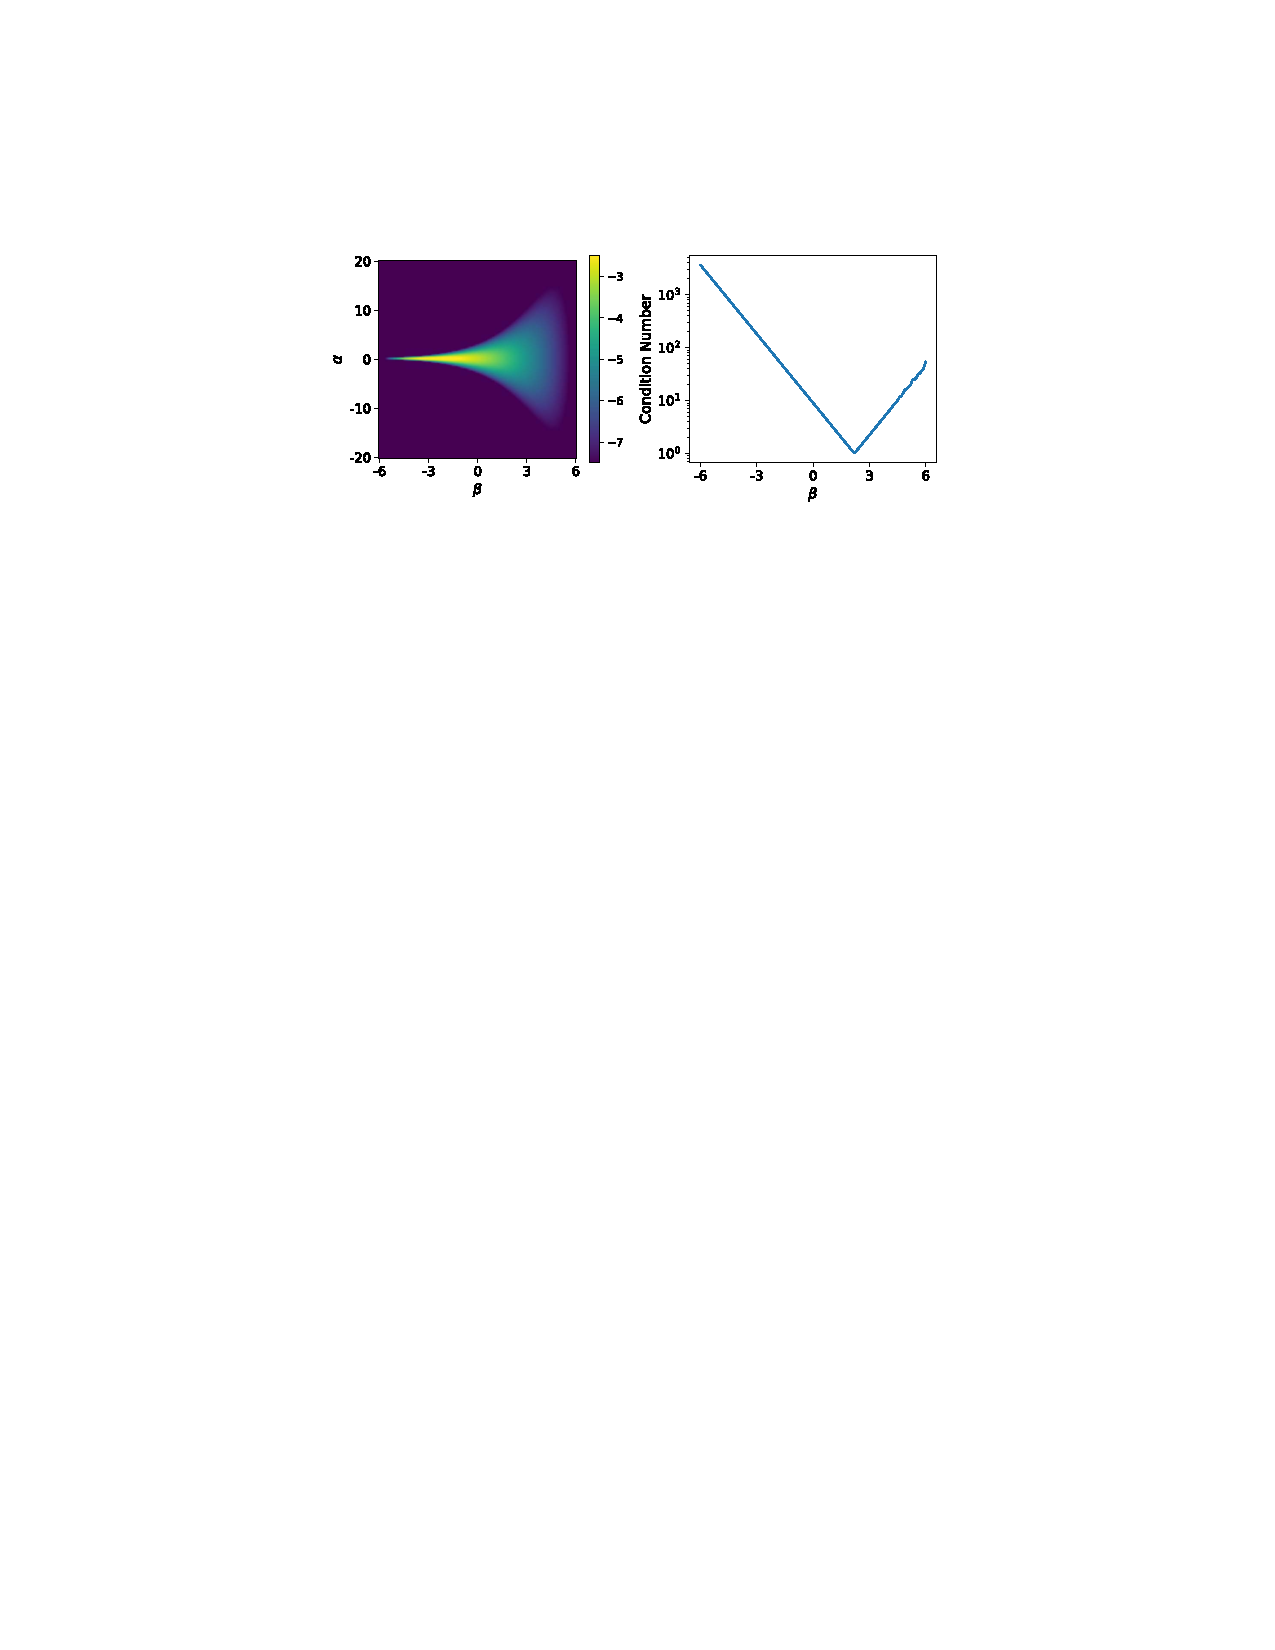
\includegraphics[width=3.25in]{img/funnel-condition.pdf}
\end{center}

\sld{Hamiltonian dynamics}
\begin{itemize}
\item \myemph{Potential energy} at $\theta \in \mathbb{R}^D$ is negative log density $U(\theta) = -\log
  \left( \strut p(\theta \mid y) \right)$.
\item \myemph{Kinetic energy} for momentum $\rho \in \mathbb{R}^D$ is
  $V(\rho) = -\log \left( \strut \textrm{normal}(\rho \mid 0, 1) \right).$
\item \myemph{Hamiltonian} is sum $H(\theta) = U(\theta) + V(\theta)$
\item \myemph{Leapfrog step} for Hamiltonian dynamics w.\
discretization time $\epsilon > 0$
\begin{align*}
  \rho_{t+1/2} &= \rho_t - \frac{\epsilon}{2} \cdot \nabla U(\theta)
  \\
  \theta_{t + 1} &= \theta_t - \epsilon \cdot \nabla V(\theta)
  \\
  \rho_{t+1} &= \rho_{t + 1/2} - \frac{\epsilon}{2} \cdot \nabla U(\theta)
\end{align*}
\item \myemph{Precondition} with pos.\ def.\ metric $\Sigma$ by $V(\rho) =
  -\log \left( \strut \textrm{normal}(\rho \mid 0, Sigma) \right).$
\end{itemize}

\sld{Hamiltonian Monte Carlo (HMC)}
\begin{itemize}
\item \myemph{Input}: initial position $\draw{\theta}{0}$, step size
  $\epsilon$, steps $L$, metric $\Sigma$, sample size $M$
\item For each iteration $m \in 1, \ldots, M$
  \begin{subitemize}
  \item (Gibbs) Resample momentum $\rho \sim \textrm{normal}(0, \Sigma)$
  \item (Metropolis) Run leapfrog algorithm $L$ steps from $(\draw{\theta}{m-1}, \underbrace{-\rho}_{\textrm{flip}})$
    to $(\theta^*, \rho^*)$
  \item  \vspace*{-6pt} $\textrm{accept} = \textrm{uniform}(0, 1)
    < \textrm{min}\left(1, \frac{\displaystyle \strut \exp(-H(\theta^*, \rho^*))}
           {\displaystyle \strut \exp(-H(\draw{\theta}{m-1},
             \rho))}\right)$
  \vspace*{6pt}
  \item $(\draw{\theta}{m}, \draw{\rho}{m}) = (\theta^*, \rho^*)$
         if \ $\textrm{accept}$ \ else $(\draw{\theta}{m-1}, \draw{\rho}{m-1})$.
  \end{subitemize}
\item \myemph{Output}: sample $\draw{\theta}{1}, \ldots, \draw{\theta}{M}$
  \vfill
\item \myemph{Generalized HMC}: Partially resample $\rho \sim
  \textrm{normal}\!\left( \sqrt{1 - \lambda} \cdot \draw{\rho}{m-1}, \ \lambda \cdot \Sigma \right).$
\end{itemize}

\sld{HMC fails on the funnel}
\begin{itemize}
\item \myemph{Fixed step size} leads to \myemph{truncated sampling}
  with HMC (and NUTS), either
  \begin{subitemize}
    \item \myemph{Neck}: step size too big, \myemph{Hamiltonian diverges} and we \myemph{reject}.
    \item \myemph{Mouth}: step size too small, \myemph{diffusion too slow}.
      explore.
    \item Result is \myemph{biased estimation} of quantities of interest.
    \end{subitemize}
  \item Vertical dashed lines show the left truncation (color = step size)
\end{itemize}
\begin{center}
  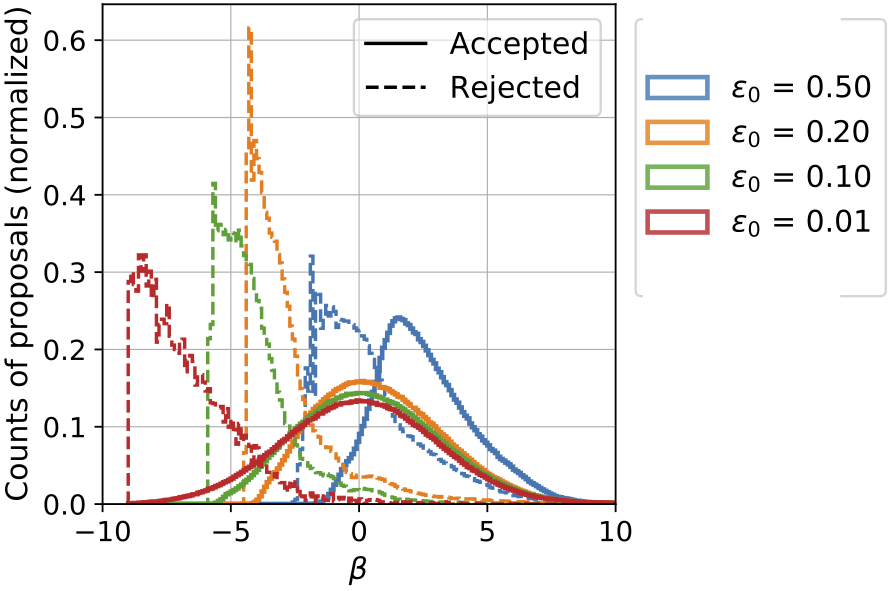
\includegraphics[width=1.75in]{img/hmc-rejections.png}
\end{center}

\sld{HMC works, but generalized HMC fails}
\begin{itemize}
\item \myemph{HMC scales in dimension} by making \myemph{directed
    progress} per iteration
\item \myemph{Hamiltonian flow} keeps trajectory in region of high probability
\item Leapfrog integrator is \myemph{symplectic}
  \begin{subitemize}
  \item preserves Hamiltonian well, so \myemph{high Metropolis accept} rate
  \item it's \textit{not} an accurate ODE solver (but that's OK)
  \end{subitemize}
\vspace*{-8pt}
\item \myemph{G-HMC reverts to random walk} because of the \myemph{flipped momentum}
  \begin{subitemize}
  \item G-HMC usually configured to use \myemph{one leapfrog step}
    (like MALA)
  \item required to preserve stationarity (cf. 100\% refreshed in standard HMC) 
  \item \myemph{reverses momentum} on failure, so need \myemph{sequences of acceptances}
  \item need large step size to move, small step sizes for acceptance
  \end{subitemize}
\end{itemize}

\sld{Dramatis Personae}
\begin{center}
  \begin{tabular}{cccc}
    
\includegraphics[width=0.85in]{img/turok.png}
    & 
\includegraphics[width=0.85in]{img/modi.png}
    & 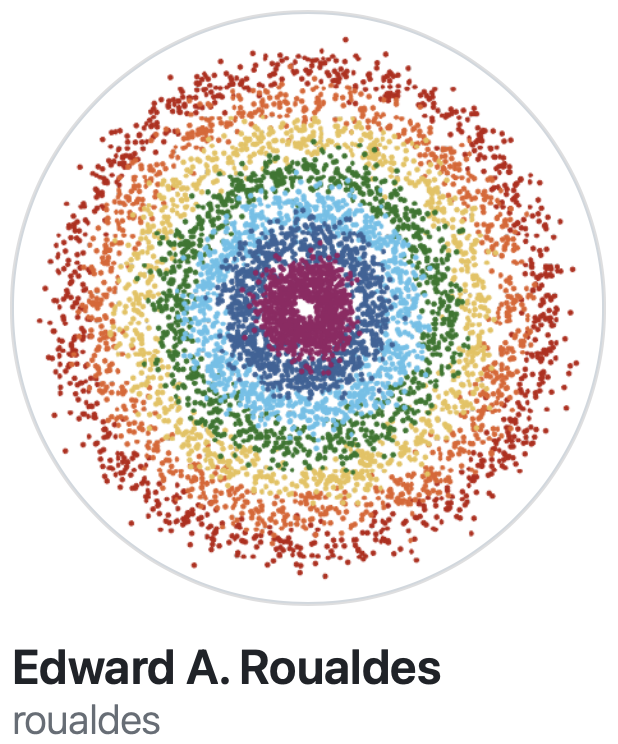
\includegraphics[width=0.85in]{img/roualdes.png}
    & 
\includegraphics[width=0.85in]{img/barnett.png}
    \\
    
\includegraphics[width=0.85in]{img/neal.png}
    & 
\includegraphics[width=0.85in]{img/hoffman.png}
    & 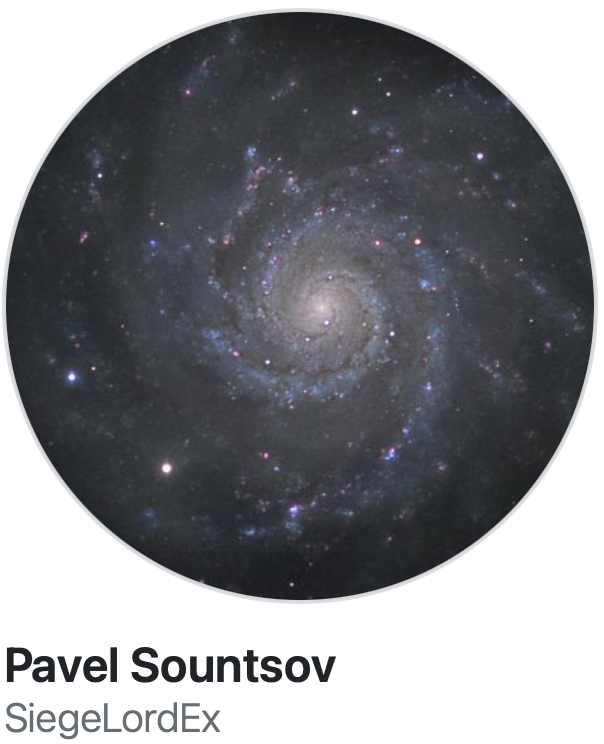
\includegraphics[width=0.85in]{img/sountsov.png}
  \end{tabular}
\end{center}




\sld{References}
\begin{itemize}
\item Modi, C., Barnett, A. and Carpenter, B., 2023. \myemph{Delayed rejection
  Hamiltonian Monte Carlo for sampling multiscale
  distributions}. \textit{Bayesian Analysis}.
\item Hoffman, M.D. and Sountsov, P., 2022. \myemph{Tuning-free
  generalized Hamiltonian Monte Carlo}.  \textit{AISTATS}.
\item Neal, R.M., 2020.  \myemph{Non-reversibly updating a uniform [0, 1] value
  for Metropolis accept/reject decisions}. \textit{arXiv}.
\end{itemize}

\end{document}
